\chapter{Òrbita el·líptica heliocèntrica}

El primer pas en la resolució de la trajectòria interplanetària és l'obtenció dels elements de l'òrbita que porta la nau d'un planeta a l'altre. Per tal de conèixer aquests elements és necessari saber quins són els punts d'origen i de destí de la nau. És a dir, cal saber la posició dels planetes en l'instant en què la sonda surt del planeta d'origen i en l'instant en què arriba al planeta de destí. Coneixent aquestes dues posicions ja és possible projectar una òrbita com la que es veu en la figura \ref{esquema_orb}.

\begin{figure}[H]
	\centering
	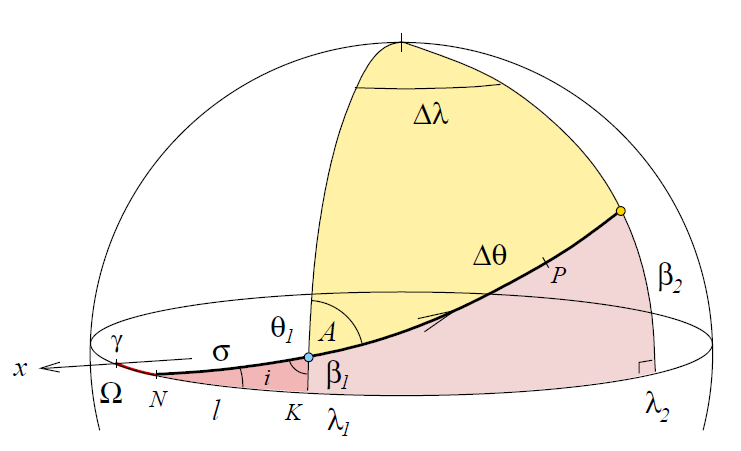
\includegraphics[scale=0.7]{./plots/esquema_orbi}
	\caption{Òrbita interplanetària heliocèntrica del planeta d'origen al planeta de destí}
	\label{esquema_orb}
\end{figure}

\section{Plantejament d'equacions}
Com es dedueix de la figura, és possible calcular la inclinació de l'òrbita sabent la posició dels dos planetes. A partir dels vectors de posició, es pot calcular la desviació respecte de l'eclíptica dels planetes d'origen (en blau) i de destí (en groc), $\beta_{1}$ i $\beta_{2}$ respectivament. També es pot obtenir la longitud eclíptica dels dos planetes, $\lambda_{1}$ i $\lambda_{2}$. A partir d'aquestes variables, el problema es resol aplicant trigonometria esfèrica:
\begin{equation}
\cos\Delta\theta=\sin\beta_{1}\sin\beta_{2}+\cos\beta_{1}\cos\beta_{2}\cos\Delta\lambda
\end{equation}
Del triangle groc s'obté:
\begin{equation}
\sin A=\cos\beta_{2}\frac{\sin\Delta\lambda}{\sin\Delta\theta}
\end{equation}

\begin{figure}[H]
	\centering
	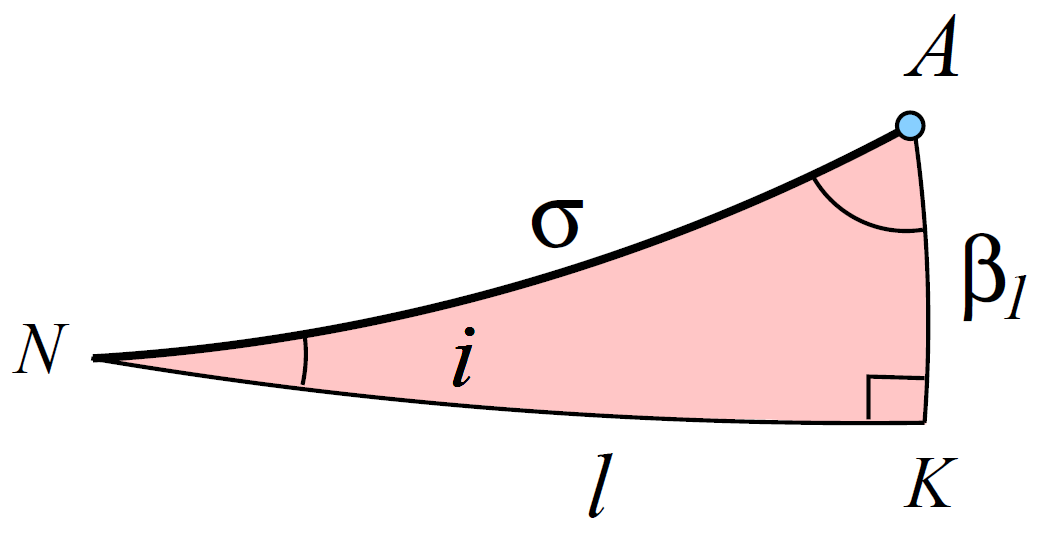
\includegraphics[scale=0.3]{./plots/triangle}
	\caption{Triangle esfèric de l'òrbita interplanetària heliocèntrica}
	\label{triang}
\end{figure}

D'altra banda, del triangle esfèric de la figura \ref{triang} s'obtenen les següents expressions:
\begin{equation}
\tan\sigma=\frac{\cos\beta_{1}}{\tan\beta_{1}}
\end{equation}
\begin{equation}
\cos i=\sin A\cos\beta_{1}
\label{eqi}
\end{equation}
\begin{equation}
\sin l=\frac{\tan\beta_{1}}{\tan i}
\end{equation}

De la figura \ref{esquema_orb} també es poden deduir l'ascensió recta del node ascendent i l'argument del perigeu:
\begin{equation}
\Omega=\lambda_{1}-l
\label{eqOmega}
\end{equation}
\begin{equation}
\omega=2\pi-\left(\theta_{1}-\sigma\right)
\label{eqw}
\end{equation}

Finalment, a partir dels vectors de posició també s'obtenen els tres elements orbitals que falten. Assumint que la trajectòria és el·líptica, els mòduls dels vectors de posició vénen donats per les expressions:
\begin{equation}
r_{1}=\frac{a\left(1-e^{2}\right)}{1+e\cos\theta_{1}}
\end{equation}
\begin{equation}
r_{2}=\frac{a\left(1-e^{2}\right)}{1+e\cos\left(\theta_{1}+\Delta\theta\right)}
\end{equation}
D'altra banda, també es pot relacionar el temps amb la posició de la sonda en l'òrbita mitjançant l'equació:
\begin{equation}
\frac{2\pi t}{T}=2\arctan\left(\sqrt{\frac{1-e}{1+e}}\tan\frac{\theta_{1}}{2}\right)-\frac{e\sqrt{1-e^{2}}\sin\theta_{1}}{1+e\cos\theta_{1}}
\end{equation}
on $T$ és el període en dies del planeta d'origen.

Per tant, es pot plantejar un sistema de tres equacions amb tres incògnites:
\begin{equation}
e=\frac{r_{2}-r_{1}}{r_{1}\cos\theta_{1}-r{2}\cos\left(\theta_{1}+\Delta\theta\right)}
\label{eqe}
\end{equation}
\begin{equation}
a=\frac{r_{1}\left(1+e\cos\theta_{1}\right)}{1-e^{2}}
\label{eqa}
\end{equation}
\begin{multline}
	t_{2}-t_{1}=\frac{365.25}{2\pi}a^{3/2}\cdot \\
	\cdot\left[2\arctan\left(\sqrt{\frac{1-e}{1+e}}\tan\frac{\left(\theta_{1}+\Delta\theta\right)}{2}\right)-\frac{e\sqrt{1-e^{2}}\sin\left(\theta_{1}+\Delta\theta\right)}{1+e\cos\left(\theta_{1}+\Delta\theta\right)}\right]- \\
	-2\arctan\left(\sqrt{\frac{1-e}{1+e}}\tan\frac{\theta_{1}}{2}\right)-\frac{e\sqrt{1-e^{2}}\sin\theta_{1}}{1+e\cos\theta_{1}}
	\label{eqt}
\end{multline}
en què tant els vectors $\vec{r_{1}}$ i $\vec{r_{2}}$ com el semieix major $a$ estan expressats en AU, per tal de treballar amb valors més simples.

\section{Mètode de resolució}
\begin{enumerate}
	\item Es calcula la posició del planeta d'origen en l'instant de temps de sortida i la posició del planeta de destí en l'instant de temps d'arribada.
	\item A partir dels vectors de posició es calculen les longituds i latituds eclíptiques dels planetes.
	\item A partir del sistema d'equacions donat per \ref{eqe}, \ref{eqa} i \ref{eqt} s'obtenen l'excentricitat $e$ i el semieix major $a$ de l'òrbita, i l'anomalia vertadera de la sonda $\theta_{1}$ en l'instant de sortida.
	\item Es calcula la inclinació a partir de les equacions donades pels triangles esfèrics \ref{eqi}.
	\item Càlcul de la longitud eclítpica del node ascendent donat per \ref{eqOmega}.
	\item Es calcula l'argument del periheli amb \ref{eqw}.
\end{enumerate}